\paragraph{Generalisation.} \Cref{thm:generalization} controls the uniform
deviation over the score class. On SL-Bench (\cref{app:scaling}) it decays with
exponent $\nExpFiveDevRate$ against the $-\tfrac12$ the bound predicts, every
cell in $[\nExpFiveRateMin,\nExpFiveRateMax]$. Regressing the fitted
$n^{-1/2}$ coefficient on $\log\Gamma$ gives $R^{2}=\nExpFiveRtwoLog$; on
$\Gamma$, $R^{2}=\nExpFiveRtwoLin$. Over a $\nExpFiveGammaRange$-fold range of
$\Gamma$ the coefficient grows by $\nExpFiveCoefGrowthPct\%$ --- consistent
with the $\log\Gamma$ of \cref{cor:loggamma} and not with a linear dependence,
which would predict more than an order of magnitude. The \emph{excess risk of
the empirical minimiser} decays much faster (exponent $\nExpFiveExcessRate$):
the familiar fast-rate phenomenon for a strongly convex objective, consistent
with an upper bound without being evidence for its rate, which is why we
measure the uniform deviation instead.

\paragraph{Uncertainty.} \Cref{fig:uq} and \cref{app:uq-table} separate three
things. \emph{Identification.} With oracle nuisances every claim of
\cref{cor:uq} holds: $p_1(x)$ lies inside the identified set for
$\nExpThreeOracleInBox$ of units at every $n$, and the naive aleatoric
estimate overstates the truth by $\nExpThreeAleaBias$ nats (about
$\nExpThreeAleaBiasRelPct\%$) while sitting inside the identified interval,
where no test on observed data can refute it. \emph{Asymptotic
overconfidence.} For a converged ensemble the reported epistemic term falls by
$\nExpThreeEpiDrop\times$ between $n=2{,}000$ and $n=70{,}000$ (fitted exponent
$\nExpThreeSlopeLog$), while the censoring term moves by
$\nExpThreeCensChangePct$ with no trend; at the largest sample the ratio is
$\nExpThreeRatioLast$: the reported uncertainty is two orders of magnitude
smaller than the identification uncertainty it omits. \emph{A
different, detectable pathology.} A fixed-budget deep ensemble's ``epistemic''
term does not contract (exponent $\nExpThreeSlopeMlp$) and exceeds the
censoring term throughout, but that is optimisation noise: its calibration
error is $\nExpThreeCalRatioMlpOverLog\times$ larger, and a calibration check
catches it, unlike the bias of \cref{cor:uq}.

\begin{figure}[t]
\centering
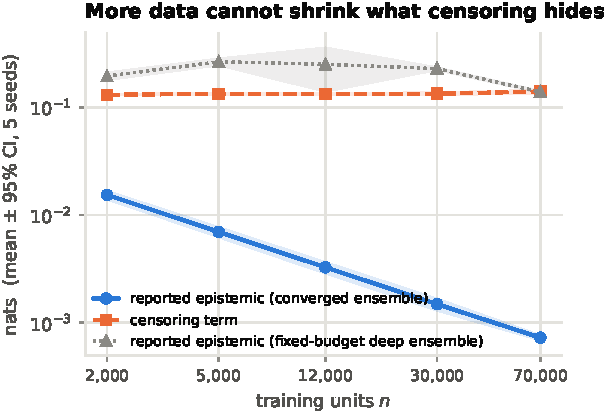
\includegraphics[width=0.58\linewidth]{figures/fig4_uq}
\caption{\textbf{More data cannot shrink what censoring hides}
(\cref{cor:uq}; $\nExpThreeSeeds$ seeds, 95\% bands). The reported epistemic
term of a converged ensemble collapses; the censoring term \eqref{eq:cens}
does not. A fixed-budget deep ensemble's term does not collapse either, for an
unrelated reason --- optimisation noise --- which a calibration check detects.}
\label{fig:uq}
\end{figure}
